
\begin{Large}
\begin{center}
\textbf{INFORME SERVICIO MYSQL} \\
\end{center}
\end{Large}

\section{Objetivos - INFORME SERVICIO MYSQL} 


\begin{itemize}

Implementar el servicio MySQL en un servidor CentOS de Linux para la administración de base de datos.\\

\end{itemize} 

\section{Recursos Necesarios} 

\begin{itemize}
\item Para MV-CentOS6.2-SO2
\\- Una computadora con capacidad para virtualizar en hardware.
\\-	Un mínimo de 2 GB de RAM.
\\-	Disco duro dedicado de por lo menos 60 GB.
\\-	Instalador en formato ISO de CentOS 6.2.
\\\
\end{itemize} 

\begin{itemize}
\item Para MV-WXP-SO2
\\- Una computadora con capacidad para virtualizar en hardware.
\\-	Un mínimo de 1 GB de RAM.
\\-	Disco duro dedicado de por lo menos 60 GB.
\\-	Instalador en formato ISO de Windows XP SP3.
\\\
\end{itemize} 

\begin{itemize}
\item Para MV-W8.1-SO2
\\- Una computadora con capacidad para virtualizar en hardware.
\\-	Un mínimo de 4 GB de RAM.
\\-	Disco duro dedicado de por lo menos 60 GB.
\\-	Instalador en formato ISO de Windows 8.1.
\\\
\end{itemize} 

\section{Marco Teórico} 
\begin{itemize}
\item Concepto de MySQL
\\ MySQL, es un sistema de gestión de base de datos relacional o SGBD. Este gestor de base de datos en multihilo y multiusuario, lo que le permite ser utilizado por varias personas al mismo tiempo, e incluso, realizar varias consultas a la vez, lo que lo hace sumamente versátil.

Nació como una iniciativa de Software Libre y aún sigue ofreciéndose como tal, para usuarios particulares. Pero si se desea utilizarlo para promover datos en una empresa, se puede comprar una licencia, como un software propietario, que es autoría de la empresa patrocinante (Actualmente Oracle Corporation).\\
\end{itemize} 

\begin{itemize}
	\begin{center}
		
\includegraphics[width=10cm]{./Imagenes/1a}
		\end{center}
\end{itemize} 

\begin{itemize}
\item Utilidad de MySQL
\\ Como comentábamos anteriormente este gestor de base de datos es muy utilizado en desarrollo web, ya que permite a los desarrolladores y diseñadores, realizar cambios en sus sitios de manera simple, con tan sólo cambiar un archivo, evitando tener que modificar todo el código web. Esto se debe a que MySQL, trabaja con un sistema centralizado de gestión de datos, que permite realizar cambios en un solo archivo y que se ejecuta en toda la estructura de datos que se comparte en la red. Además, permite incluir noticias e información rápidamente en un sitio web, utilizando un simple formulario, sin tener que tocar el código del website.

Cuando se combina con PHP, se convierte en una mezcla poderosa, que siempre es tomada en cuenta para realizar aplicaciones cliente/servidor, que requieran el uso de una base de datos rápida, segura y potente.\\
\end{itemize} 

\begin{itemize}
\item Algunas características de MySQL
\\- Autenticación de usuarios con permisos específicos para ciertas bases de datos, atadas a las direcciones IP de origen.
\\-	Gestión de memoria y cache para una cantidad determinada de consultas o transacciones simultáneas.
\\-	Conectores para integración en ambientes PHP, Perl, Pyton, ODBC.
\\-	Replicación transaccional en línea de la base de datos, a otra base paralela.
\\- Monitoreo de usuarios, transacciones, uso de memoria  y de procesos.
\\- Uso de triggers o disparadores para actuar sobre creación, edición o borrado de registros.
\\- Uso automático de valores autonuméricos en las tablas.
\\- Se pueden crear vistas, procedimientos almacenados y funciones.
\\- Posee funciones de chequeo del desempeño de consultas y sus índices, cómo también de los parámetros de memoria, caché, transacciones, etc. Podemos encontrar un consejero de desempeño en Phpmyadmin.
\\- Se puede administrar desde consola, phpmyadmin, o desde programas externos como MySQLfront o Sequel (para MacOS) mediante conexión por el puerto TCP 3306.
\\- Puede manejar millones de registros en una sola tabla.
\\- Gestiona el bloqueo de tablas para evitar conflictos de transacciones simultáneas.
\\- Se pueden importar o exportar datos o la estructura misma de la base, sus tablas, índices, etc
\\\
\end{itemize}

\section{Desarrollo} 
\begin{itemize}
	\begin{center}
		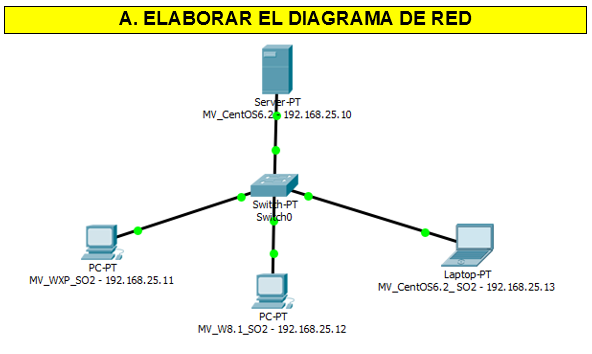
\includegraphics[width=13cm]{./Imagenes/2a}
		\end{center}
\end{itemize} 

\begin{itemize}
	\begin{center}
		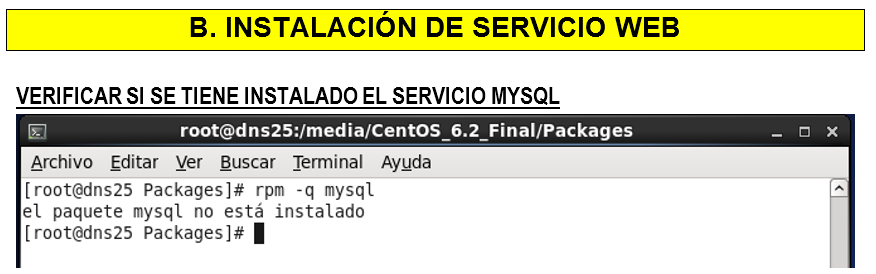
\includegraphics[width=13cm]{./Imagenes/3a}
		\end{center}
\end{itemize} 

\begin{itemize}
	\begin{center}
		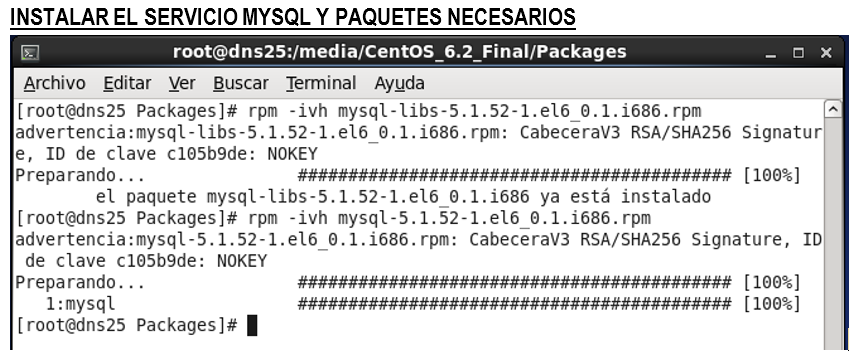
\includegraphics[width=13cm]{./Imagenes/4a}
		\end{center}
\end{itemize} 

\begin{itemize}
	\begin{center}
		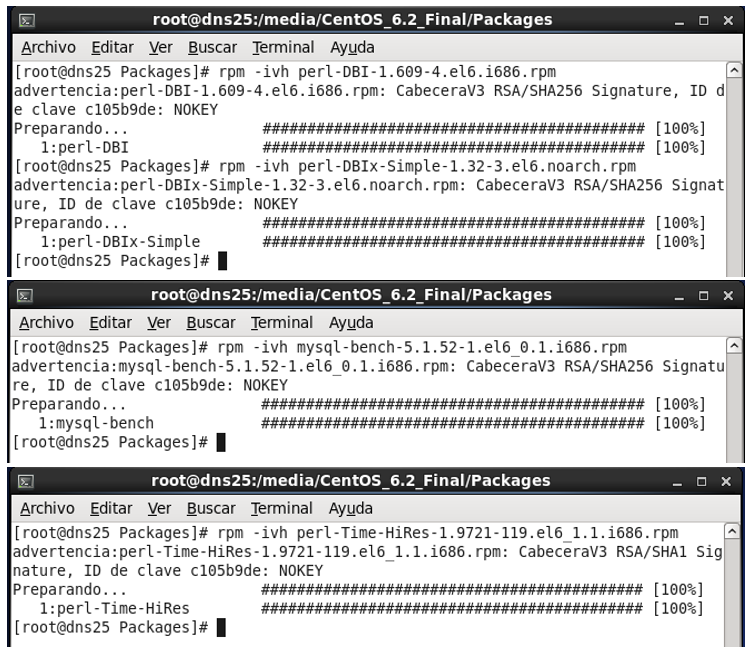
\includegraphics[width=13cm]{./Imagenes/5a}
		\end{center}
\end{itemize} 

\begin{itemize}
	\begin{center}
		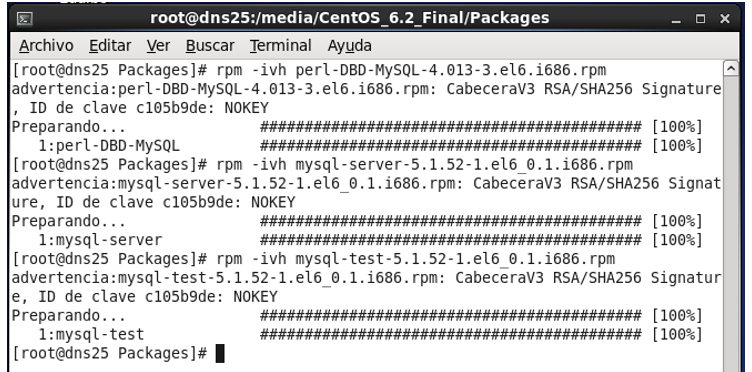
\includegraphics[width=13cm]{./Imagenes/6a}
		\end{center}
\end{itemize} 

\begin{itemize}
	\begin{center}
		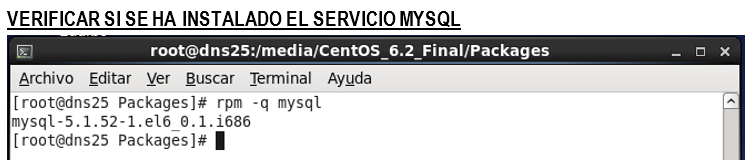
\includegraphics[width=13cm]{./Imagenes/7a}
		\end{center}
\end{itemize} 

\begin{itemize}
	\begin{center}
		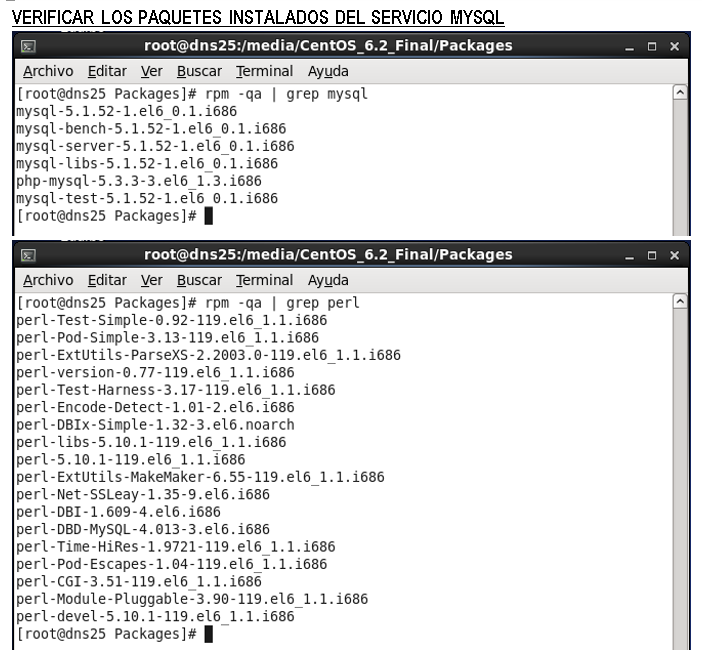
\includegraphics[width=13cm]{./Imagenes/8a}
		\end{center}
\end{itemize} 

\begin{itemize}
	\begin{center}
		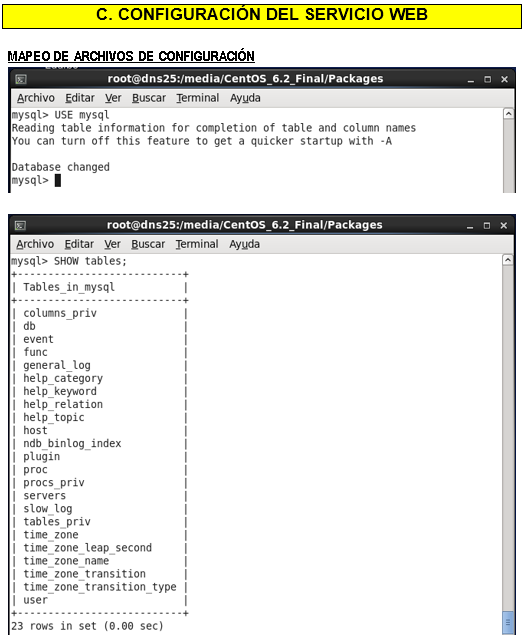
\includegraphics[width=13cm]{./Imagenes/9a}
		\end{center}
\end{itemize} 

\begin{itemize}
	\begin{center}
		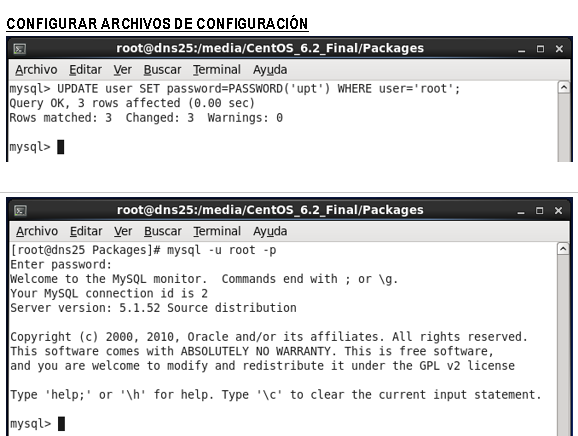
\includegraphics[width=13cm]{./Imagenes/10a}
		\end{center}
\end{itemize} 

\begin{itemize}
	\begin{center}
		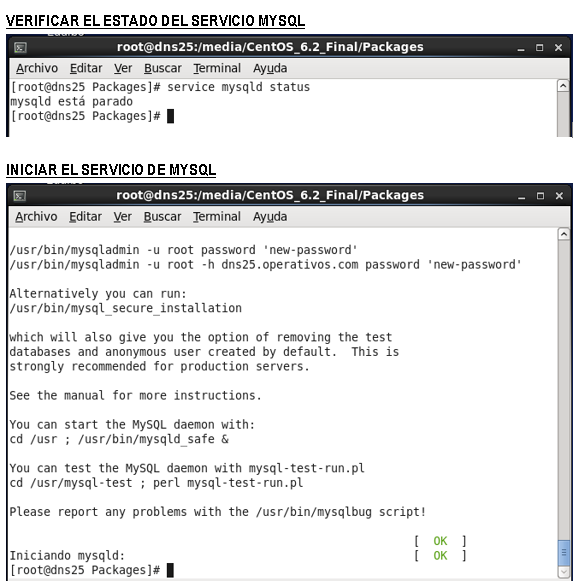
\includegraphics[width=13cm]{./Imagenes/11a}
		\end{center}
\end{itemize} 

\begin{itemize}
	\begin{center}
		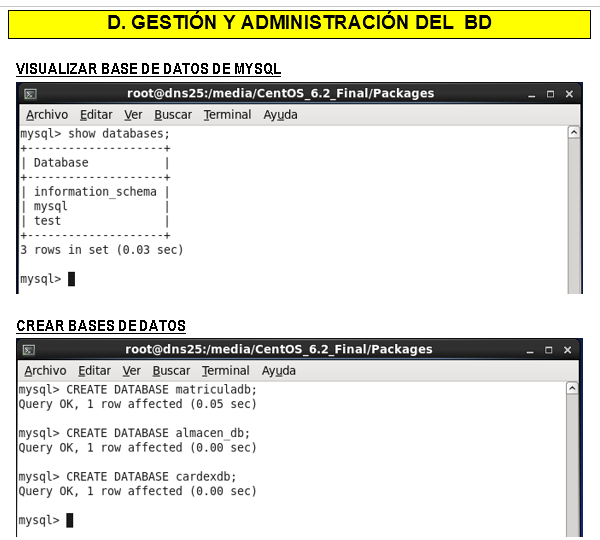
\includegraphics[width=13cm]{./Imagenes/12a}
		\end{center}
\end{itemize} 

\begin{itemize}
	\begin{center}
		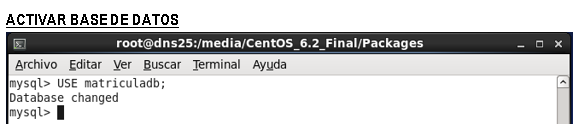
\includegraphics[width=13cm]{./Imagenes/13a}
		\end{center}
\end{itemize} 

\begin{itemize}
	\begin{center}
		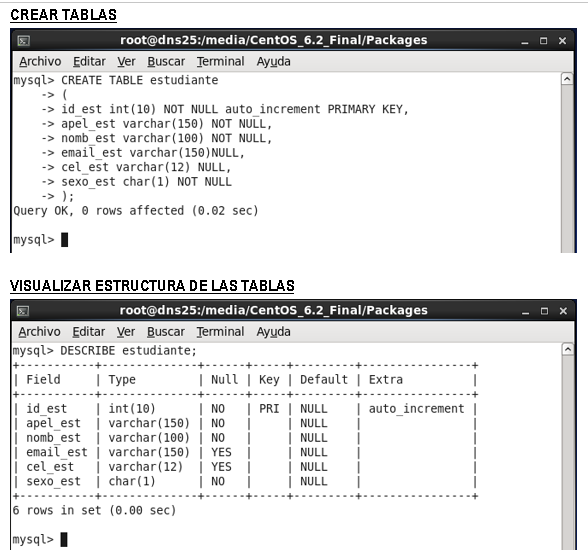
\includegraphics[width=13cm]{./Imagenes/14a}
		\end{center}
\end{itemize} 

\begin{itemize}
	\begin{center}
		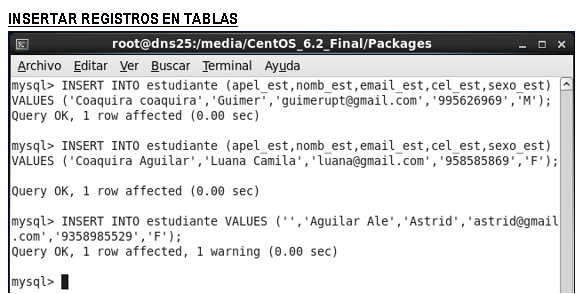
\includegraphics[width=13cm]{./Imagenes/15a}
		\end{center}
\end{itemize} 

\begin{itemize}
	\begin{center}
		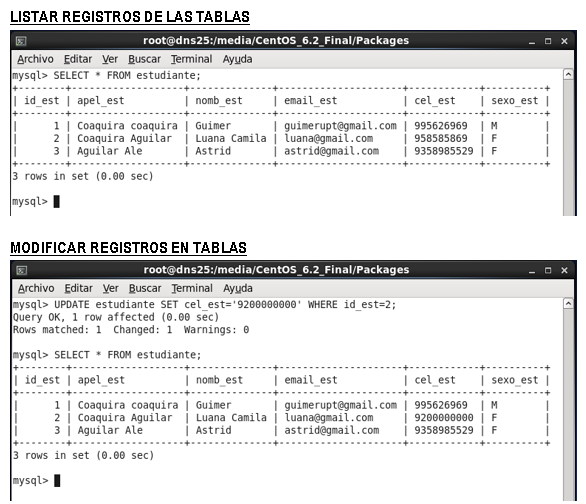
\includegraphics[width=13cm]{./Imagenes/16a}
		\end{center}
\end{itemize} 

\begin{itemize}
	\begin{center}
		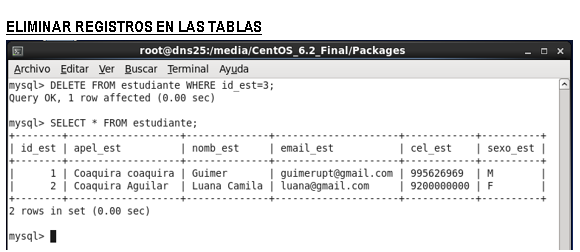
\includegraphics[width=13cm]{./Imagenes/17a}
		\end{center}
\end{itemize} 

\begin{itemize}
	\begin{center}
		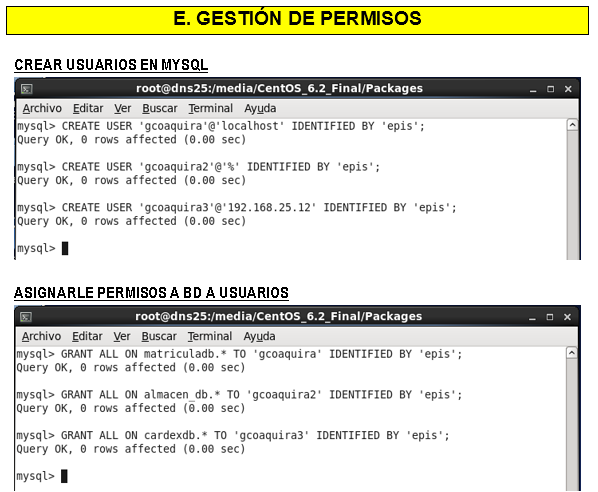
\includegraphics[width=13cm]{./Imagenes/18a}
		\end{center}
\end{itemize} 

\begin{itemize}
	\begin{center}
		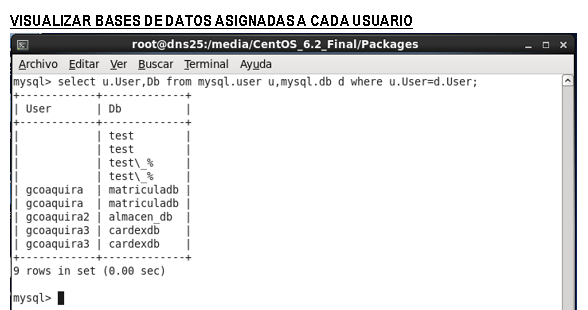
\includegraphics[width=13cm]{./Imagenes/19a}
		\end{center}
\end{itemize} 

\begin{itemize}
	\begin{center}
		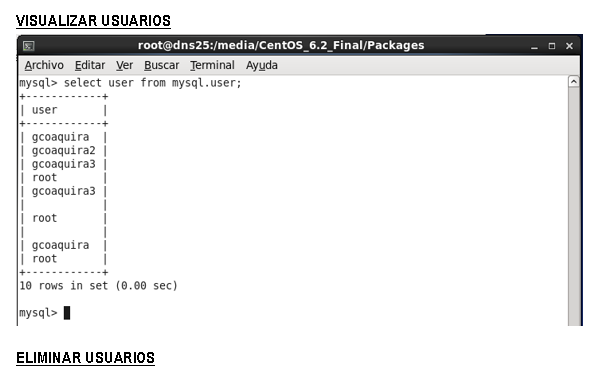
\includegraphics[width=13cm]{./Imagenes/20a}
		\end{center}
\end{itemize} 

\begin{itemize}
	\begin{center}
		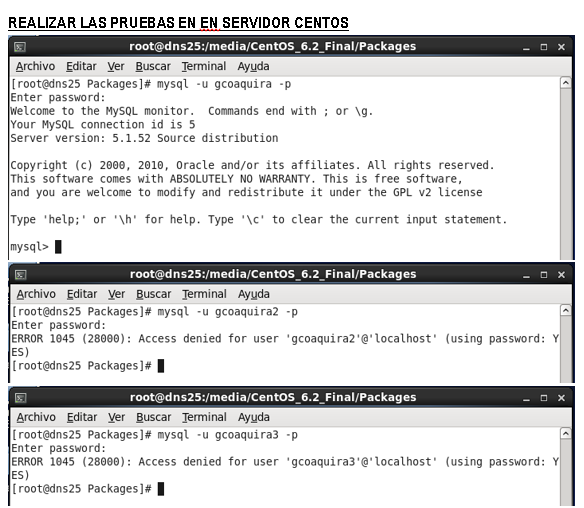
\includegraphics[width=13cm]{./Imagenes/21a}
		\end{center}
\end{itemize} 

\begin{itemize}
	\begin{center}
		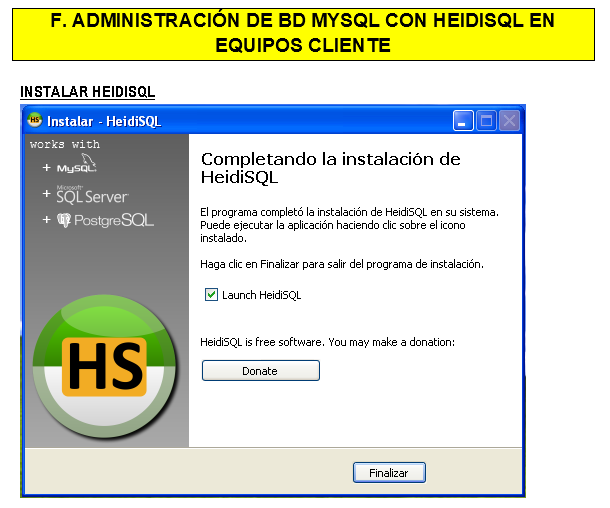
\includegraphics[width=13cm]{./Imagenes/22a}
		\end{center}
\end{itemize} 

\begin{itemize}
	\begin{center}
		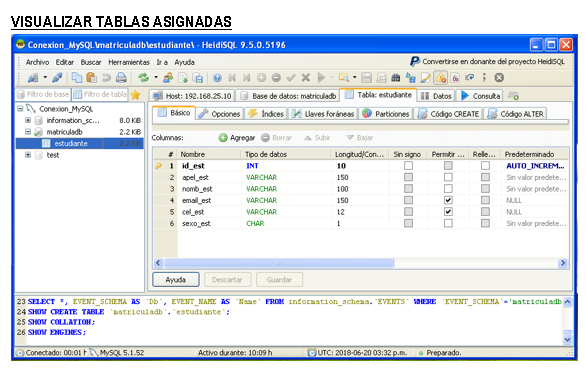
\includegraphics[width=13cm]{./Imagenes/23a}
		\end{center}
\end{itemize} 